\subsection*{Single Shot MultiBox Detector}

Zwar liefern die oben genannten Objektdetektoren akkurate Ergebnisse, allerdings sind sie als zu rechenintensiv und langsam einzuordnen, als dass sie für Echtzeit Applikationen eingesetzt werden könnten. Der \textit{Single Shot MultiBox Detector} (SSD) unterschiedet sich von vorhergehenden Modellen, wie beispielsweise den R-CNN Detektoren, dahingehend, dass er bewusst auf den Schritt der Generierung von Bounding Box Vorschlägen und des \textit{Poolings} verzichtet, um wesentlich schneller ablaufen zu können als andere Objektdetektoren. Die Präzision der Klassifikationen bleibt hierbei erhalten, selbst Bilder niedriger Auflösung können weiterhin verarbeitet werden. Dem \textit{SSD} genügt also ein einziges tiefes neuronales Netz zum Lokalisieren und Klassifizieren von Objekten. Wie der \textit{SSD} aufgebaut ist und welche Ansätze er verfolgt, soll in diesem Unterkapitel erläutert werden \cite{ssd.20161229}. 

\begin{figure}[ht]
	\begin{center}
		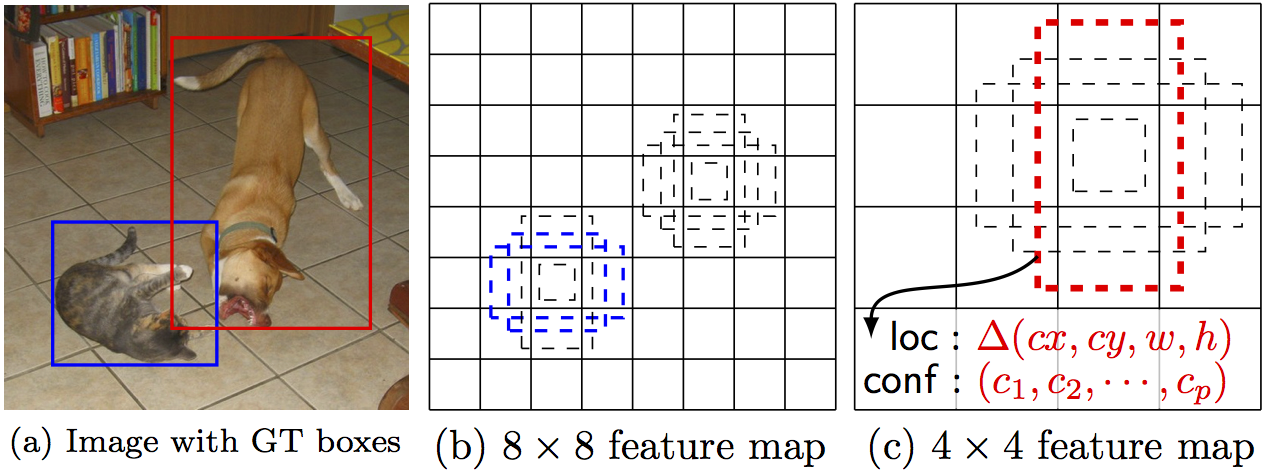
\includegraphics[width=15cm]{Bilder/ssd_framework.png} 
		\caption[SSD Grundprinzip]{SSD Grundprinzip \cite{ssd.20161229}}
		\label{framework}
	\end{center}
\end{figure}

Die Architektur des \textit{SSD} zielt zunächst darauf ab, ein Bild in mehrere unterschiedliche Gitterstrukturen zu unterteilen, die sich nach ihrer Skalierung unterscheiden. Dadurch ist es möglich Objekte unterschiedlicher Größe zu erkennen. Jede Lokation im Gitter besitzt eine gleiche Anzahl an festen, vordefinierten Bounding Boxen, die unterschiedliche Seitenverhältnisse aufweisen (siehe Abbildung \ref{framework}). So wird sichergestellt, dass sowohl horizontal als auch vertikal ausgeprägte Objekte in der selben Lokation gleichzeitig erkannt werden können (siehe Abbildung \ref{boundingboxes}) \cite{ssd.20161229}.

\begin{figure}[ht]
	\begin{center}
		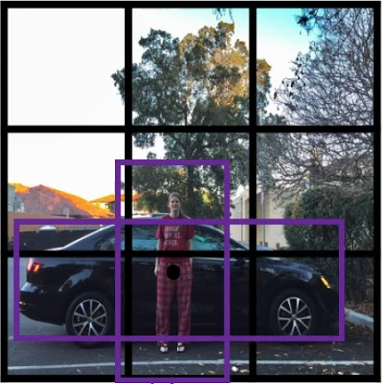
\includegraphics[width=7cm]{Bilder/bounding_boxes.png} 
		\caption[Bounding Boxes]{Bounding Boxes \cite{AndrewNg.2019}}
		\label{boundingboxes}
	\end{center}
\end{figure}

Für jede dieser Bounding Boxen bestimmt der \textit{SSD} Wahrscheinlichkeiten für Klassenzugehörigkeiten als auch Verschiebungen der vordefinierten Bounding Box zur wahren Bounding Box des Objekts für jede Klasse. Dies wird mit kleinen Faltungsfiltern erreicht, die in den hinteren Schichten des Netzwerks eingesetzt werden \cite{ssd.20161229}.

Die Kostenfunktion ist durch die gewichtete Summe des Lokalisationsverlustes und des Klassifikationsverlustes bestimmt. Während der Klassifikationverlust durch eine \textit{Softmax} Funktion bestimmt werden kann, wird der Lokalisationsverlust über die \textit{Smooth L1} Funktion (\ref{smooth}) bestimmt \cite{ssd.20161229}.

\begin{equation}\label{smooth}
\begin{split}
L_{loc}(t^u,v) = \sum\limits_{i \in (x,y,w,h)}^{n} SM_{L1}(t^u_i - v_i) \\
SM_{L1}(t^u_i - v_i) = \begin{cases}
							0.5x^2      & \text{wenn } |x| < 1\\
							|x| - 0.5   & \text{sonst}
						   \end{cases}
\end{split}
\end{equation}
\equations{Die Smooth L1 Funktion}

\begin{figure}[ht]
	\begin{center}
		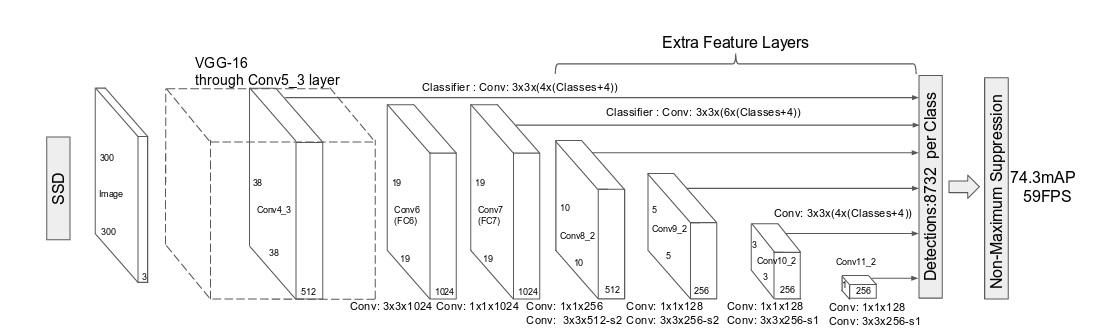
\includegraphics[width=15cm]{Bilder/ssd_architecture.png} 
		\caption[SSD Architektur]{SSD Architektur \cite{ssd.20161229}}
		\label{architecture}
	\end{center}
\end{figure}

Der \textit{SSD} benutzt ein \textit{VGG-16} Basis Netzwerk, um Klassifikationen zu ermöglichen. \textit{VGG-16} ist ein auf dem Datensatz von \textit{ImageNet} basierendes neuronales Netz, das bis zu 1000 unterschiedliche Kategorien klassifizieren kann \cite{MathWorks.2019b}. Unabhängig vom Basisnetzwerk werden Convolutional Layer als Hilfsstrukturen zur Objektdetektion eingesetzt. Diese verarbeiten die Bilder unterschiedlicher Gittergrößen, wobei die Gittergröße mit fortschreitenden Convolutional Layern abnimmt. Jeder Convolutional Layer kann eine feste Anzahl an Detektionen bestimmen. Eine Detektion wird durch eine Klassenangabe und die Lage einer vorhergesagten Bounding Box bestimmt. Eine Bounding Box wird durch einen Eckpunkt $P(x,y)$ und eine Höhe und Breite bestimmt. Bei $c$ Klassen hat der Ausgangsvektor demnach die Größe $c+4$. Für jede vordefinierte Bounding Box werden, falls vorhanden, die Koordinaten der originalen Bounding Box ermittelt dabei relativ zur vordefinierten Bounding Box abgespeichert. Die Zuordnung einer Bounding Box zu einer vordefinierten Bounding Box erfolgt über die sogenannte \textit{Intersection over Union} (IoU) (siehe Abbildung \ref{iou}). Überschreitet diese einen Wert von 0.5, so ist diese der originalen Bounding Box zugeordnet \cite{ssd.20161229}. Demnach ist es möglich, dass eine originale Bounding Box mehreren vordefinierten Bounding Boxen zugeordnet werden kann \cite{ssd.20161229} .

\begin{figure}[ht]
	\begin{center}
		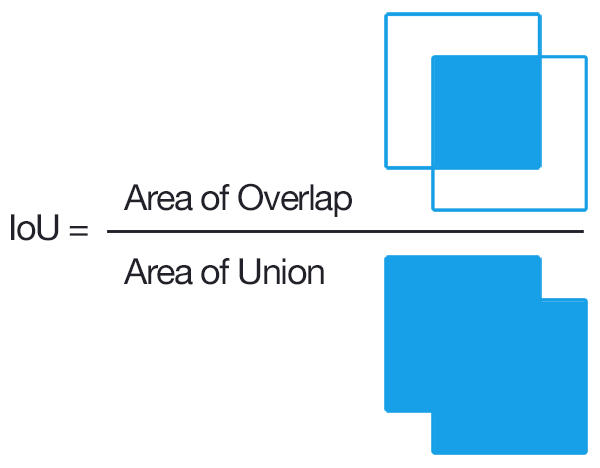
\includegraphics[width=8cm]{Bilder/iou_equation.png} 
		\caption[Intersection over Union]{Intersection over Union \cite{AdrianRosebrock.20161107}}
		\label{iou}
	\end{center}
\end{figure}

Bei $m \cdot n$ Lokationen und $k$ verschiedenen vordefinierten Bounding Boxen pro Lokation ergeben sich also $m \cdot n \cdot k \cdot (c+4)$ verschiedene Werte für eine Feature Map. Die Merkmalsextraktion zur Klassifikation wird durch Faltung mit $3x3$ Filtern erreicht \cite{ssd.20161229}.

Dieser Vorgang wird für alle Feature Maps für alle Convolutional Layer durchgeführt. Die daraus folgende Menge an Detektionen wird durch ein \textit{Non Maximum Suppression Layer} in ihrer Größe reduziert. Als Maß zur Filterung wird die sogenannte \textit{Intersection over Union} (IoU) der detektierten Box zur wahren Box verwendet \cite{ssd.20161229}.

Während der Trainingsprozesses des \textit{SSD300}\footnote{SSD300 verwendet Bilder der Auflösung 300x300 Pixel. Alternativ existiert ebenso SSD512 für Bilder der Auflösung 512x512 Pixel. Die Bilder können jedoch auch kleiner als die vorgegebene Auflösung gewählt werden.} mit PASCAL VOC2007 wurde eine Lernrate von $\eta = 10^{-3}$ für das Mini-Batch Verfahren mit Batchgröße 32 und Moment $\beta = 0.9$ verwendet. Die Gewichtungen wurden \textit{Xavier} initialisiert. Nach 40.000 Iterationen wurde die Lernrate für 10.000 Iterationen auf $\eta = 10^{-4}$ reduziert und schließlich auf $\eta = 10^{-5}$ \cite{ssd.20161229}. 

\begin{figure}[ht]
	\begin{center}
		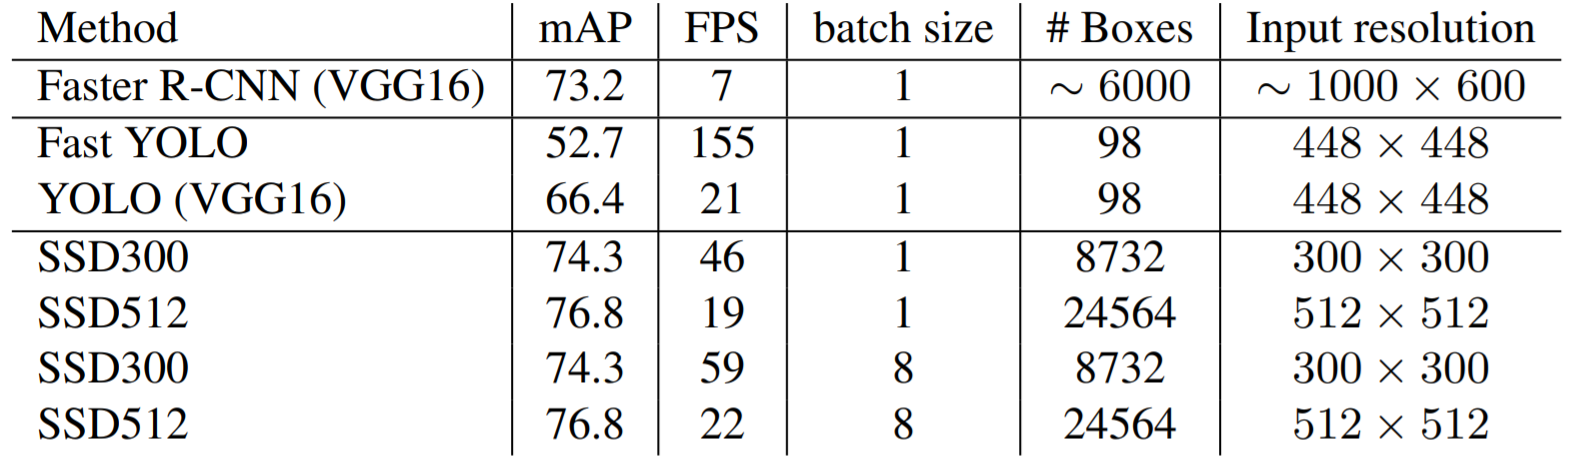
\includegraphics[width=12cm]{Bilder/ssd_results.png} 
		\caption[Vergleich SSD]{Vergleich SSD \cite{ssd.20161229}}
		\label{result}
	\end{center}
\end{figure}

Nach obiger Grafik ist eindeutig festzustellen, dass \textit{SSD300} ein gutes Verhältnis zwischen Präzision und Reaktionsvermögen bewahrt. Durch den Verzicht auf den Schritt der Generierung von Bounding Box Vorschlägen und des \textit{Poolings} kann \textit{SSD} deutlich schneller ablaufen als die Vergleichsdetektoren, während durch das Vordefinieren von Bounding Boxen ebenso eine hohe Präzision erzielt werden kann \cite{ssd.20161229}.

Allerdings ergibt sich vor allem für kleine Objekte ein erschwertes Detektionsvermögen, da diese in den höherliegenden Convolutional Layern untergehen. Als Lösung hierfür kann eine erhöhte Inputgröße gewählt werden (vgl. \textit{SSD512}) oder Daten-Augmentierung für den Lernprozess angewandt werden. Weitere mögliche Fehler können falsche Positivbefunde aufgrund von fehlerhafter Lokalisation sein, Verwechslung mit ähnlichen Kategorien oder dem Hintergrund sowie weitere \cite{ssd.20161229}.

Letztendlich lässt sich \textit{SSD} als schneller Objektdetektor beurteilen, der nicht nur einfach zu trainieren und integrieren ist, sondern ebenso ein gutes Verhältnis zwischen Lokalisationspräzision und Echtzeitvermögen schafft.
